\subsubsection{Q10.20 data 11092021 grouped by scenario \& x_first}

\begin{comment}
                     EFPR        EO      EFNR     n    pvalue
(frauth, False)  0.409091  0.590909  0.363636  11.0  0.682007
(frauth, True)   0.545455  0.454545  0.590909  11.0  0.676575
(icu, False)     0.409091  0.590909  0.636364  11.0  0.818546
(icu, True)      0.666667  0.333333  0.666667   6.0  0.275234
(rent, False)    0.250000  0.750000  0.562500   8.0  0.045500
(rent, True)     0.550000  0.450000  0.350000  10.0  0.916512
\end{comment}

\begin{table}[h]
    \centering
    \begin{tabular}{|c|c|c|c|c|c|c|}
        \hline
        scenario & x_first & EFPR & EO & EFNR & n & p-value\\
        \hline
        frauth & False & 0.409 & \textbf{0.591} & 0.364 & 11.0 & 0.682\\
		frauth & True & \textbf{0.545} & 0.455 & \textbf{0.591} & 11.0 & 0.677\\
		icu & False & 0.409 & \textbf{0.591} & \textbf{0.636} & 11.0 & 0.819\\
		icu & True & \textbf{0.667} & 0.333 & \textbf{0.667} & 6.0 & 0.275\\
		rent & False & 0.250 & \textbf{0.750} & \textbf{0.562} & 8.0 & \textbf{0.046}\\
		rent & True & \textbf{0.550} & 0.450 & 0.350 & 10.0 & 0.917\\
		
        \hline
    \end{tabular}
    \caption{Grouped by scenario x_first}
    \label{tab:my_label}
\end{table}
\begin{figure}[h]
    \centering
    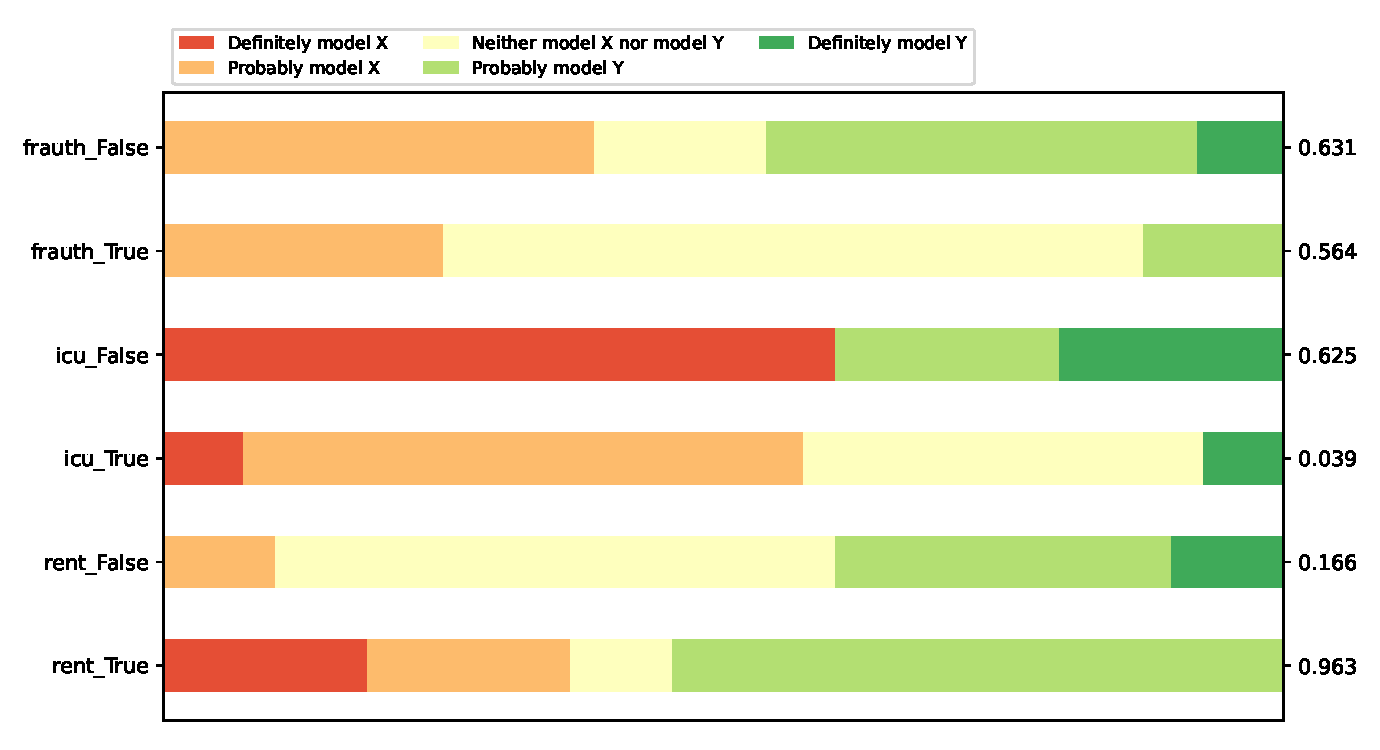
\includegraphics[width=0.8\textwidth]{figures/Q10.20/11092021/Q10.20_scenario_x_first.pdf}
    \caption{Grouped by scenario \& x_first}
    \label{fig:my_label}
\end{figure}
